\documentclass[11pt,a4paper]{article}

\usepackage[margin=2.3cm, headheight=14pt]{geometry}
\usepackage[T1]{fontenc}
\usepackage[utf8]{inputenc}
\usepackage{lmodern}
\usepackage{amsmath,amssymb}
\usepackage{graphicx}
\graphicspath{{figures/}{assessment/CW02/figures/}}
\usepackage{booktabs}
\usepackage{array}
\usepackage{enumitem}
\usepackage{fancyhdr}
\usepackage{hyperref}
\usepackage{xcolor}
\setlength{\parindent}{0pt}
\setlength{\parskip}{0.55em}
\setlength{\emergencystretch}{2.5em}

\hypersetup{
    colorlinks=true,
    linkcolor=blue!60!black,
    urlcolor=blue!60!black,
}

% Right-aligned mark tag on its own line matching UCL COMP0037 coursework style
\newcommand{\qmarks}[1]{\par\nopagebreak\noindent\hfill\mbox{\textbf{[#1 marks]}}}
\newcommand{\qtotal}[1]{\par\smallskip\noindent\hfill\textbf{[Total #1 marks]}\par\medskip}

% UCL-style running footer ("TURN OVER" on odd pages, "CONTINUED" on even pages)
\pagestyle{fancy}
\fancyhf{}
\renewcommand{\headrulewidth}{0pt}
\renewcommand{\footrulewidth}{0.4pt}
\fancyfoot[L]{\thepage}
\fancyfoot[R]{\ifodd\value{page} TURN OVER \else CONTINUED \fi}

\fancypagestyle{endpage}{
    \fancyhf{}
    \renewcommand{\headrulewidth}{0pt}
    \renewcommand{\footrulewidth}{0.4pt}
    \fancyfoot[L]{\thepage}
    \fancyfoot[R]{END OF COURSEWORK}
}

\begin{document}

% --------------------------------------------------------------------------- %
% Title block (matching COMP0037 2026/27 Coursework 1)
% --------------------------------------------------------------------------- %
\begin{center}
    {\LARGE \textbf{COMP0037 2026/27 Coursework 2}}\\[0.5em]
    {\large COMP0037 Teaching Team}\\[0.3em]
    {\normalsize Term 2, AY 2026/27}
\end{center}

\section*{Overview}
\begin{itemize}[leftmargin=1.5em, itemsep=0.25em]
    \item \textbf{Coursework 02 Release Date:} \textit{TBD (Week 7)}
    \item \textbf{Assignment Due Date:} \textit{TBD (End of Module --- after Week 9, 16:00 UK time)}
    \item \textbf{Weeks Covered:} Weeks 06--09 (Learning from Demonstration, LLM Task Planning, Vision-Language-Action Models, and Safe System Integration)
    \item \textbf{Weighting:} 60\% of the module total (Assessment Type: AT10 / GN02 --- Group Coursework with End-Point Submission)
    \item \textbf{Recommended Length:} 3,000--3,500 words per group (excluding figures, tables, equations, references, and appendices)
    \item \textbf{Final Submission Format.} Each group must submit two things:
    \begin{enumerate}[label=\arabic*., leftmargin=1.8em, itemsep=0.2em]
        \item A zip file (which contains the source code implemented to tackle this coursework). The name of the zip file must be of the form \texttt{COMP0037\_CW2\_GROUP\_g.zip}, where \texttt{g} is the letter/number code of your group.
        \item A report in PDF format. It must be named \texttt{COMP0037\_CW2\_GROUP\_g.pdf}.
    \end{enumerate}
    \textit{Note that a penalty of 2\% will be applied if the files are submitted with the wrong name.}
\end{itemize}

\section*{Mark Allocation and Further Instructions}
The total marks for each question are written in the form \textbf{[X marks]}. The coursework is marked out of \textbf{100 marks}. Approximately \textbf{65\%} of the total coursework marks are awarded for your analysis and \textbf{35\%} for your coding of the algorithms. Therefore, please take time and care with your writing, experimental design, and analysis of solutions.

For the submitted code, you must use the notation, variable names, and code structure provided in the lectures and the coursework starter kit (\texttt{cw2\_starter/}, available on Moodle). If you do not use these, we will consider the work a potential plagiarism case and investigate further.

This coursework introduces a new \textbf{mobile manipulation (loco-manipulation)} environment and dual-table sample-transfer task distinct from the fixed-base tabletop tasks in the weekly lab sessions; you will adapt and extend the methods learned in Labs 06--09 to solve it. Areas requiring implementation are indicated with \texttt{TODO(CW2-...)} comments.

As discussed in Lecture 00 (Overview), we expect you to take care in writing your report:
\begin{itemize}[leftmargin=1.5em, itemsep=0.2em]
    \item Figures and graphs must be numbered, labelled, and have informative captions.
    \item Equations must be typeset (e.g., via \LaTeX{} or an equation editor). Equations captured by a screenshot from the slides or elsewhere are of low quality and are likely to incur a mark penalty.
    \item When we ask you to write or modify code, provide a clear explanation in your report of what you wrote and why.
    \item Include a \textbf{Reproducibility Block} (exact commands, seeds, Python, PyTorch, Robosuite, and MuJoCo versions, and CPU/GPU hardware or Colab runtime) and a \textbf{Signed Group Contribution Table} (Appendix~A, excluded from the word count) documenting each member's primary workstream and peer-verification role.
\end{itemize}

The final mark will be computed by summing all marks awarded on individual questions out of 100. The code will not be independently marked but must be provided before the submission deadline. It may be executed during marking, and if it does not run or fails to reproduce the results presented in the report, this will impact your marks.

\newpage

% --------------------------------------------------------------------------- %
% Use Case
% --------------------------------------------------------------------------- %
\section*{Use Case}
Continuing the \textbf{MedBot} hospital automation scenario from Coursework~1, the hospital pharmacy now deploys a \textbf{wheeled mobile manipulator} (\texttt{PandaOmron}: an Omron holonomic mobile base carrying a 7-DoF Franka Emika Panda arm with a parallel-jaw gripper) inside a dual-bench sample-processing bay (\texttt{MobilePickPlaceEnv}, defined in \texttt{cw2\_starter/mobile\_pick\_place\_env.py}).

\begin{figure}[htbp]
    \centering
    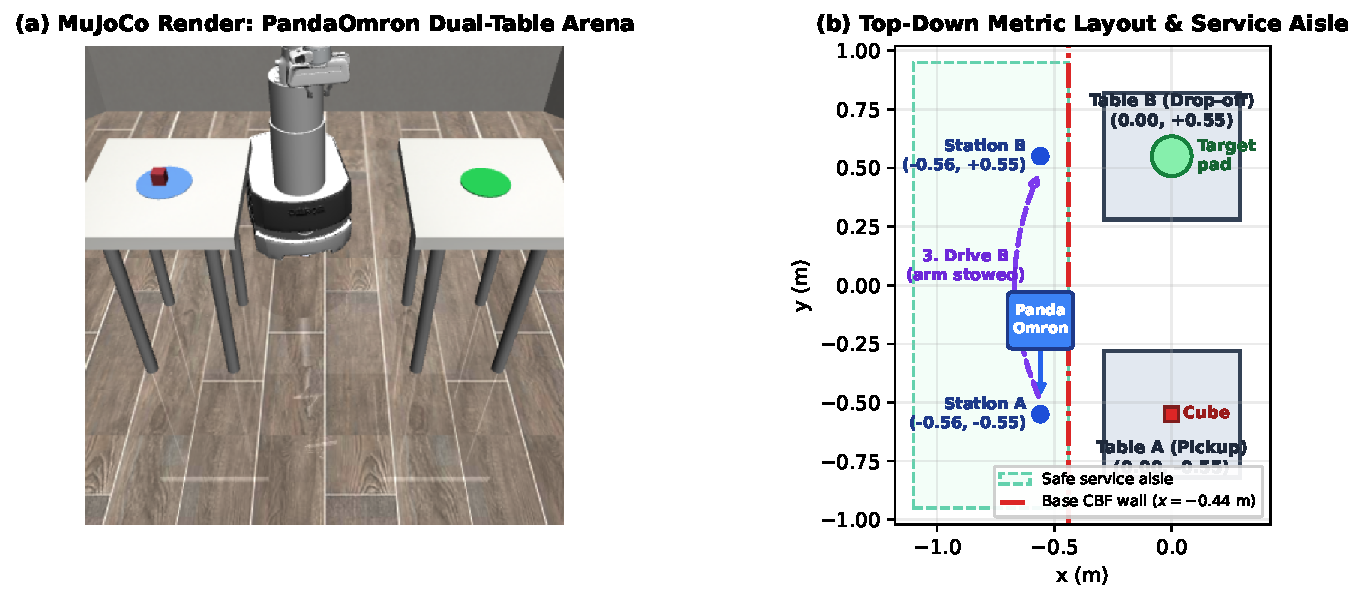
\includegraphics[width=\textwidth]{figures/fig1_mobile_arena.pdf}
    \caption{The \texttt{MobilePickPlaceEnv} dual-table pharmacy bay (\texttt{cw2\_starter/mobile\_pick\_place\_env.py}): (a)~Robosuite/MuJoCo \texttt{agentview} render of \texttt{PandaOmron} in the service aisle facing Table~A (pickup bench with red specimen cube) and Table~B (drop-off bench with green target pad); (b)~top-down metric layout showing Station~A ($x=-0.56,\,y=-0.55\,$m), Station~B ($x=-0.56,\,y=+0.55\,$m), the 4-stage transfer sequence, and the base-to-table safety boundary ($x_{\max} = -0.44\,$m).}
    \label{fig:mobile_arena}
\end{figure}

In every episode, \texttt{PandaOmron} spawns in the service aisle ($x = -0.56\,$m, randomized $y_0 \in [-0.25, 0.05]\,$m) and must execute a four-stage \textbf{mobile pick-and-place transfer} using its 11-D whole-body \texttt{BASIC} composite controller ($a_{0:6}$: arm \texttt{OSC\_POSE} delta, $a_6$: torso, $a_{7:10}$: holonomic base velocity $[v_x, v_y, \omega_z]$, $a_{10}$: gripper):
\begin{enumerate}[label=\arabic*., leftmargin=1.8em, itemsep=0.18em]
    \item \textbf{Navigate to Station~A:} Drive the mobile base along the aisle to align with Table~A ($y = -0.55\,$m) while keeping the arm at safe transit height.
    \item \textbf{Pick Specimen Cube:} Hover, descend, grasp, and lift the red specimen cube (randomized $(x, y)$ offset on Table~A).
    \item \textbf{Transport to Station~B:} Drive the mobile base along the aisle to Table~B ($y = +0.55\,$m) without dropping the cube or colliding with either bench.
    \item \textbf{Place on Target Pad:} Lower the cube onto the green target pad on Table~B, open the gripper, and retract cleanly.
\end{enumerate}

% --------------------------------------------------------------------------- %
% Part 1
% --------------------------------------------------------------------------- %
\section*{Part 1}
In this part (Weeks 06--07), you compare imitation learning from whole-body demonstrations with structured symbolic task planning over closed-loop mobile-manipulation skills.

\begin{enumerate}[label=\textbf{\arabic*.}, leftmargin=1.4em, itemsep=1.0em]

% --- Question 1 ---
\item To bootstrap autonomous sample transfer without hand-crafting a reward function, the team collects whole-body demonstrations from the 8-phase scripted Finite-State Machine (FSM) expert in \texttt{cw2\_starter/q1\_mobile\_lfd.py}.
\begin{enumerate}[label=\textbf{\alph*.}, leftmargin=1.6em, itemsep=0.45em]
    \item Explain the \textbf{Behavioral Cloning (BC)} supervised imitation-learning objective and derive why BC suffers from quadratic error compounding $O(\epsilon H^2)$ under \textbf{covariate shift}. Explain why this failure mode is amplified in mobile manipulation (where base-alignment errors propagate into end-effector grasp misses) compared to fixed-base tabletop grasping, and how input-noise augmentation or DAgger mitigates it. \qmarks{7}

    \item Complete \texttt{train\_bc} and \texttt{evaluate\_bc\_policy} in \texttt{cw2\_starter/q1\_mobile\_lfd.py} to train a Behavioral Cloning MLP mapping the 16-D proprioceptive state (\texttt{extract\_proprio}) to 11-D whole-body \texttt{PandaOmron} actions, supporting optional Gaussian state-noise augmentation (\texttt{noise\_std}) during training. Explain your network architecture, feature normalization, and training setup. \qmarks{9}

    \item Run a controlled evaluation on \texttt{MobilePickPlaceEnv} comparing: (i)~BC dataset-size scaling across $N \in \{4, 8, 16\}$ expert demonstrations, (ii)~Standard BC vs.\ Noise-Augmented BC (\texttt{noise\_std = 0.01}) on nominal episodes (\texttt{cube\_xy\_noise = 0.04\,m}), and (iii)~both policies under out-of-distribution cube perturbations (\texttt{cube\_xy\_noise = 0.08\,m}). Present training curves, success rates, final cube-to-pad distances, and rollout visualizations, and diagnose the dominant failure modes. \qmarks{9}
\end{enumerate}
\qtotal{25}

% --- Question 2 ---
\item Rather than learning a single end-to-end policy, an alternative architecture decomposes mobile manipulation into a \textbf{Large Language Model (LLM) Task Planner} driving a typed \textbf{Mobile-Manipulation Skill API} (\texttt{MobileSkillLibrary} in \texttt{q2\_mobile\_llm\_planner.py}).

\begin{enumerate}[label=\textbf{\alph*.}, leftmargin=1.6em, itemsep=0.45em]
    \item Explain why exposing a robot through a \textbf{typed, schema-constrained skill API} with explicit symbolic preconditions is safer and more reliable than asking an LLM to output raw joint or Cartesian velocities directly. Identify three mobile-manipulation-specific failure modes (e.g., driving while the arm is extended over a table) that symbolic preconditions can catch before actuation. \qmarks{7}

    \item Complete \texttt{validate\_plan} and \texttt{MobileLLMPlanner.plan} in \texttt{q2\_mobile\_llm\_planner.py}. Your validator must verify both JSON schema conformance and symbolic preconditions across the sequence (\texttt{arm\_stowed} before \texttt{drive\_to\_station}, docked at Station~\texttt{A} before \texttt{pick\_cube}, docked at Station~\texttt{B} and \texttt{holding\_cube} before \texttt{place\_cube}). Explain your symbolic state transition rules and closed-loop failure recovery loop. \qmarks{9}

    \item Evaluate your validator on a battery of valid and adversarial/malformed plans (unknown skill, driving before stowing, picking from the aisle, placing without holding the cube), and execute your planner in closed loop on \texttt{MobilePickPlaceEnv}. Report per-skill step counts, end-to-end transfer success, and discuss what happens when a physical grasp slips mid-transit and \texttt{verify\_grasp()} triggers replanning. \qmarks{9}
\end{enumerate}
\qtotal{25}

\newpage

% --------------------------------------------------------------------------- %
% Part 2
% --------------------------------------------------------------------------- %
\section*{Part 2}
In this part (Weeks 08--09), you build a self-contained Vision-Language-Action (VLA) diffusion policy from scratch and integrate a coupled Whole-Body Control Barrier Function (CBF) safety shield with red-teaming validation.

% --- Question 3 ---
\item To enable visuomotor control directly from onboard RGB images, you adapt the \textbf{Track~A VLA} pipeline (\texttt{cw2\_starter/q3\_mobile\_vla.py}) combining a miniature Vision-Language Model (\texttt{NanoVLM}) with a \textbf{Conditional Diffusion Action Head} executed in closed loop.
\begin{enumerate}[label=\textbf{\alph*.}, leftmargin=1.6em, itemsep=0.45em]
    \item Explain four design choices from the VLA architecture: (i)~$2\times 2$ \textbf{pixel-shuffle token compression}, (ii)~\textbf{prefix-concat attention masking} (including why a float $0$/$-\infty$ mask avoids validation \texttt{NaN}s compared to a boolean mask), (iii)~\textbf{DDPM diffusion} over MSE regression, and (iv)~4-step \textbf{action chunking} with receding-horizon execution. \qmarks{6}

    \item Complete \texttt{PixelShuffleProjector.forward} and \texttt{build\_prefix\_causal\_mask} in \texttt{cw2\_starter/q3\_mobile\_vla.py}. Train \texttt{NanoVLM} from scratch on $64\times 64$ \texttt{agentview} RGB frames paired with the three templated mobile-manipulation QA pairs per frame, and compare held-out exact-match VQA accuracy against the \textbf{majority-class baseline}. Explain why a small VLM can score below a majority baseline on text generation yet still supply useful visual embeddings for control. \qmarks{9}

    \item Complete \texttt{cosine\_beta\_schedule}, DDPM forward/reverse sampling, and the closed-loop evaluator \texttt{evaluate\_chunk\_mpc} to predict 4-step action chunks on the active \texttt{PandaOmron} DoFs. Run the controlled ablations on \texttt{MobilePickPlaceEnv}: (i)~undertraining (30 epochs) vs.\ converged training ($\ge 150$ epochs), (ii)~\textbf{proprioception-only} vs.\ \textbf{proprioception + frozen VLM embedding}, and (iii)~chunk execution step $k = 1$ vs.\ $k = 4$. Report training curves, closed-loop success rates, final cube-to-pad distances, and rollout visualizations. \qmarks{10}
\end{enumerate}
\qtotal{25}

% --- Question 4 ---
\item Before deploying \texttt{PandaOmron} in a shared hospital pharmacy bay, all high-level commands must pass through a \textbf{4-tier safe control stack} (\texttt{Planner} $\to$ \texttt{Skills} $\to$ \texttt{WholeBodyCBFShield} $\to$ \texttt{PandaOmron}) in \texttt{cw2\_starter/q4\_mobile\_cbf\_integration.py} (Figure~\ref{fig:wholebody_cbf}).

\begin{figure}[htbp]
    \centering
    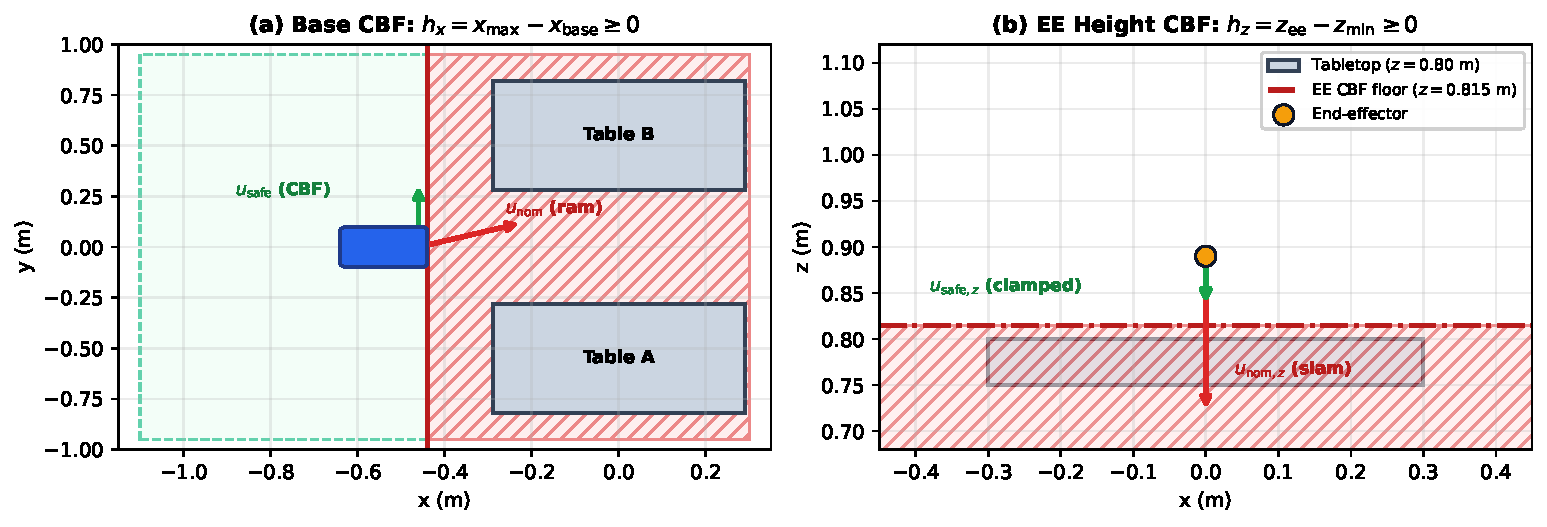
\includegraphics[width=\textwidth]{figures/fig3_wholebody_cbf.pdf}
    \caption{Coupled Whole-Body Control Barrier Function (CBF) constraints enforced by \texttt{WholeBodyCBFShield} (Question~4): (a)~top-down mobile-base barrier $h_x = x_{\max} - x_{\mathrm{base}} \ge 0$ ($x_{\max} = -0.44\,$m) preventing base collisions with Table~A and Table~B; (b)~side-view end-effector tabletop barrier $h_z = z_{\mathrm{ee}} - z_{\min} \ge 0$ ($z_{\min} = 0.815\,$m) blocking downward slams into the benches.}
    \label{fig:wholebody_cbf}
\end{figure}

\begin{enumerate}[label=\textbf{\alph*.}, leftmargin=1.6em, itemsep=0.45em]
    \item Write the discrete-time CBF condition $h(x_{t+1}) - h(x_t) \ge -\alpha\,h(x_t)$ ($\alpha \in (0, 1]$) for the mobile-base barrier $h_x(p) = x_{\max} - x_{\mathrm{base}} \ge 0$ and the end-effector barrier $h_z(e) = z_{\mathrm{ee}} - z_{\min} \ge 0$. Explain why a wheeled base requires a stopping-distance margin at $20\,$Hz, and justify the core safety principle that \textit{the planner does not have to be trustworthy if the safety filter is}. \qmarks{6}

    \item In \texttt{q4\_mobile\_cbf\_integration.py}, complete \texttt{WholeBodyCBFShield.filter\_action} and the evaluation harness \texttt{run\_red\_team\_suite} to enforce: (i)~base-to-table and aisle bounds ($x \in [-1.10, -0.44]\,$m, $y \in [-0.95, +0.95]\,$m), (ii)~end-effector tabletop clearance ($z_{\mathrm{ee}} \ge 0.815\,$m), (iii)~velocity clamping, and (iv)~a structured \texttt{SafetyAuditEntry} audit log. Explain your implementation. \qmarks{9}

    \item Compare \textbf{Unshielded} vs.\ \textbf{Whole-Body CBF Shielded} control on \texttt{MobilePickPlaceEnv} across three tests: (i)~\textbf{Nominal Transfer} (verifying that the shield preserves full task completion), (ii)~\textbf{Adversarial Ram + Slam} (commanding full-speed base ramming into the benches and downward end-effector slamming), and (iii)~\textbf{Noisy/Biased Perception \& Margin Sensitivity} (sensor calibration bias + Gaussian pose noise pushing the unshielded robot toward the tables, plus the safety-vs.-capability trade-off as $z_{\min}$ is increased). Present trajectory plots ($x_{\mathrm{base}}(t)$, $z_{\mathrm{ee}}(t)$), breach counts, and audit-log findings. \qmarks{10}
\end{enumerate}
\qtotal{25}

\end{enumerate}

\bigskip
\begin{center}
    \textbf{[Coursework 2 Total: 100 marks]}
\end{center}

\section*{Getting Help}
You are encouraged to use the Moodle assignment discussion forum when you get stuck. Please check the forum regularly and help answer each other's questions. If you have questions about this coursework, please post them on the forum rather than emailing the teaching team directly, so that all groups can see the reply.

\section*{Submission and Feedback}
The deadline for submission is \textbf{16:00 UK time} on the due date specified on Moodle. Late penalties will start to accrue if any element of the submission (report PDF or source-code ZIP) has a receipt time of 16:01 or later, following UCL's standard AT10/GN02 late-submission policy:
\begin{itemize}[leftmargin=1.5em, itemsep=0.15em]
    \item $< 2$ working days late: 10 percentage points deduction;
    \item $2$--$5$ working days late: capped at pass;
    \item $> 5$ working days late: mark of 1.00\% / Grade E.
\end{itemize}

\newpage
\thispagestyle{endpage}

% --------------------------------------------------------------------------- %
% Appendix A: Group Contribution & Peer-Verification Sign-off
% --------------------------------------------------------------------------- %
\section*{Appendix A: Group Contribution and Peer-Verification Table}
Include a completed copy of Table~\ref{tab:contributions} as the final appendix of your PDF report (excluded from the word count). Every group member must lead at least one technical workstream and peer-verify another member's code and figures.

\begin{table}[htbp]
    \centering
    \small
    \renewcommand{\arraystretch}{1.35}
    \begin{tabular}{@{} >{\raggedright\arraybackslash}p{2.3cm} >{\raggedright\arraybackslash}p{1.6cm} >{\raggedright\arraybackslash}p{5.4cm} >{\raggedright\arraybackslash}p{3.7cm} >{\raggedright\arraybackslash}p{1.5cm} @{}}
        \toprule
        \textbf{Student Name} & \textbf{UCL ID} & \textbf{Primary Workstream(s) \& Code Modified} & \textbf{Peer-Verification Role \& Report Sections} & \textbf{Sign-off} \\
        \midrule
        Member 1 & & e.g., Q1 (\texttt{q1\_mobile\_lfd.py}) & Verified Q2 code \& report & \\
        Member 2 & & e.g., Q2 (\texttt{q2\_mobile\_llm\_planner.py}) & Verified Q3 code \& report & \\
        Member 3 & & e.g., Q3 (\texttt{q3\_mobile\_vla.py}) & Verified Q4 code \& report & \\
        Member 4 & & e.g., Q4 (\texttt{q4\_mobile\_cbf\_integration.py}) & Verified Q1 code \& report & \\
        \bottomrule
    \end{tabular}
    \caption{Group contribution and peer-verification sign-off table (adapt to 3 rows for 3-student groups).}
    \label{tab:contributions}
\end{table}

\end{document}
